% Options for packages loaded elsewhere
\PassOptionsToPackage{unicode}{hyperref}
\PassOptionsToPackage{hyphens}{url}
%
\documentclass[
]{article}
\usepackage{amsmath,amssymb}
\usepackage{iftex}
\ifPDFTeX
  \usepackage[T1]{fontenc}
  \usepackage[utf8]{inputenc}
  \usepackage{textcomp} % provide euro and other symbols
\else % if luatex or xetex
  \usepackage{unicode-math} % this also loads fontspec
  \defaultfontfeatures{Scale=MatchLowercase}
  \defaultfontfeatures[\rmfamily]{Ligatures=TeX,Scale=1}
\fi
\usepackage{lmodern}
\ifPDFTeX\else
  % xetex/luatex font selection
    \setmainfont[]{Times New Roman}
\fi
% Use upquote if available, for straight quotes in verbatim environments
\IfFileExists{upquote.sty}{\usepackage{upquote}}{}
\IfFileExists{microtype.sty}{% use microtype if available
  \usepackage[]{microtype}
  \UseMicrotypeSet[protrusion]{basicmath} % disable protrusion for tt fonts
}{}
\makeatletter
\@ifundefined{KOMAClassName}{% if non-KOMA class
  \IfFileExists{parskip.sty}{%
    \usepackage{parskip}
  }{% else
    \setlength{\parindent}{0pt}
    \setlength{\parskip}{6pt plus 2pt minus 1pt}}
}{% if KOMA class
  \KOMAoptions{parskip=half}}
\makeatother
\usepackage{xcolor}
\usepackage[margin=1in]{geometry}
\usepackage{longtable,booktabs,array}
\usepackage{calc} % for calculating minipage widths
% Correct order of tables after \paragraph or \subparagraph
\usepackage{etoolbox}
\makeatletter
\patchcmd\longtable{\par}{\if@noskipsec\mbox{}\fi\par}{}{}
\makeatother
% Allow footnotes in longtable head/foot
\IfFileExists{footnotehyper.sty}{\usepackage{footnotehyper}}{\usepackage{footnote}}
\makesavenoteenv{longtable}
\usepackage{graphicx}
\makeatletter
\def\maxwidth{\ifdim\Gin@nat@width>\linewidth\linewidth\else\Gin@nat@width\fi}
\def\maxheight{\ifdim\Gin@nat@height>\textheight\textheight\else\Gin@nat@height\fi}
\makeatother
% Scale images if necessary, so that they will not overflow the page
% margins by default, and it is still possible to overwrite the defaults
% using explicit options in \includegraphics[width, height, ...]{}
\setkeys{Gin}{width=\maxwidth,height=\maxheight,keepaspectratio}
% Set default figure placement to htbp
\makeatletter
\def\fps@figure{htbp}
\makeatother
\setlength{\emergencystretch}{3em} % prevent overfull lines
\providecommand{\tightlist}{%
  \setlength{\itemsep}{0pt}\setlength{\parskip}{0pt}}
\setcounter{secnumdepth}{-\maxdimen} % remove section numbering
\ifLuaTeX
  \usepackage{selnolig}  % disable illegal ligatures
\fi
\usepackage{bookmark}
\IfFileExists{xurl.sty}{\usepackage{xurl}}{} % add URL line breaks if available
\urlstyle{same}
\hypersetup{
  pdftitle={9. Appendix},
  hidelinks,
  pdfcreator={LaTeX via pandoc}}

\title{9. Appendix}
\author{}
\date{\vspace{-2.5em}}

\begin{document}
\maketitle

\subsection{Table 1: Type A Model
Coefficients}\label{table-1-type-a-model-coefficients}

\subsubsection{Writing Score Model}\label{writing-score-model}

\begin{longtable}[]{@{}lr@{}}
\toprule\noalign{}
Covariate & Coefficient \\
\midrule\noalign{}
\endhead
\bottomrule\noalign{}
\endlastfoot
(Intercept) & 67.7019116 \\
gendermale & -9.6034239 \\
ethnic\_groupgroup B & 2.6650499 \\
ethnic\_groupgroup C & 4.6637096 \\
ethnic\_groupgroup D & 6.8989050 \\
ethnic\_groupgroup E & 12.9775727 \\
parent\_educbachelor's degree & 3.7844797 \\
parent\_educhigh school & -6.7840560 \\
parent\_educmaster's degree & 5.1368571 \\
parent\_educsome college & -1.6159435 \\
parent\_educsome high school & -6.5646825 \\
lunch\_typestandard & 1.0114546 \\
test\_prepnone & -8.8134374 \\
parent\_marital\_statusmarried & 7.4101213 \\
parent\_marital\_statussingle & -3.9987942 \\
parent\_marital\_statuswidowed & 12.3877539 \\
practice\_sportregularly & -3.4486233 \\
practice\_sportsometimes & -5.2585836 \\
is\_first\_childyes & 6.1752314 \\
transport\_meansschool\_bus & 5.9968222 \\
wkly\_study\_hours\textgreater{} 10 & -13.4167734 \\
wkly\_study\_hours10-May & -1.3229981 \\
ethnic\_groupgroup B:transport\_meansschool\_bus & -6.3830679 \\
ethnic\_groupgroup C:transport\_meansschool\_bus & -7.4764593 \\
ethnic\_groupgroup D:transport\_meansschool\_bus & -2.4486808 \\
ethnic\_groupgroup E:transport\_meansschool\_bus & -10.3029259 \\
lunch\_typestandard:practice\_sportregularly & 6.1613706 \\
lunch\_typestandard:practice\_sportsometimes & 10.0219483 \\
lunch\_typestandard:wkly\_study\_hours\textgreater{} 10 & 5.9187672 \\
lunch\_typestandard:wkly\_study\_hours10-May & -0.0747530 \\
parent\_marital\_statusmarried:is\_first\_childyes & -7.6254632 \\
parent\_marital\_statussingle:is\_first\_childyes & -0.7356701 \\
parent\_marital\_statuswidowed:is\_first\_childyes & -5.7472401 \\
parent\_marital\_statusmarried:wkly\_study\_hours\textgreater{} 10 &
10.2657209 \\
parent\_marital\_statussingle:wkly\_study\_hours\textgreater{} 10 &
18.6798500 \\
parent\_marital\_statuswidowed:wkly\_study\_hours\textgreater{} 10 &
5.9266827 \\
parent\_marital\_statusmarried:wkly\_study\_hours10-May & 3.3299876 \\
parent\_marital\_statussingle:wkly\_study\_hours10-May & 8.2992048 \\
parent\_marital\_statuswidowed:wkly\_study\_hours10-May & -0.2843766 \\
\end{longtable}

The proper interpretation of these coefficients is as follows: Holding
all other variables constant, one unit increase in {[}covariate{]} leads
to {[}coefficient{]} units increase in the outcome of interest.

\subsubsection{Math Score Model}\label{math-score-model}

\begin{longtable}[]{@{}
  >{\raggedright\arraybackslash}p{(\columnwidth - 2\tabcolsep) * \real{0.8286}}
  >{\raggedleft\arraybackslash}p{(\columnwidth - 2\tabcolsep) * \real{0.1714}}@{}}
\toprule\noalign{}
\begin{minipage}[b]{\linewidth}\raggedright
Covariate
\end{minipage} & \begin{minipage}[b]{\linewidth}\raggedleft
Coefficient
\end{minipage} \\
\midrule\noalign{}
\endhead
\bottomrule\noalign{}
\endlastfoot
(Intercept) & 43.4922358 \\
gendermale & 5.0562224 \\
ethnic\_groupgroup B & 3.1098535 \\
ethnic\_groupgroup C & 4.7866745 \\
ethnic\_groupgroup D & 4.4789082 \\
ethnic\_groupgroup E & 19.5605426 \\
parent\_educbachelor's degree & 22.6141675 \\
parent\_educhigh school & -11.9676346 \\
parent\_educmaster's degree & -1.9383911 \\
parent\_educsome college & 0.8824346 \\
parent\_educsome high school & 1.6695670 \\
lunch\_typestandard & 5.7052422 \\
test\_prepnone & -1.1067500 \\
parent\_marital\_statusmarried & 9.7201559 \\
parent\_marital\_statussingle & 3.7791454 \\
parent\_marital\_statuswidowed & 29.2537745 \\
practice\_sportregularly & -4.2708885 \\
practice\_sportsometimes & -6.0415129 \\
is\_first\_childyes & 12.5726213 \\
transport\_meansschool\_bus & 5.2495442 \\
wkly\_study\_hours\textgreater{} 10 & -4.8803371 \\
wkly\_study\_hours10-May & 4.6584310 \\
ethnic\_groupgroup B:transport\_meansschool\_bus & -4.3676804 \\
ethnic\_groupgroup C:transport\_meansschool\_bus & -7.7457168 \\
ethnic\_groupgroup D:transport\_meansschool\_bus & -0.9133233 \\
ethnic\_groupgroup E:transport\_meansschool\_bus & -10.3518240 \\
parent\_educbachelor's degree:parent\_marital\_statusmarried &
-18.4745055 \\
parent\_educhigh school:parent\_marital\_statusmarried & 0.7418296 \\
parent\_educmaster's degree:parent\_marital\_statusmarried &
1.1992797 \\
parent\_educsome college:parent\_marital\_statusmarried & -7.4231719 \\
parent\_educsome high school:parent\_marital\_statusmarried &
-8.2282777 \\
parent\_educbachelor's degree:parent\_marital\_statussingle &
-23.6303814 \\
parent\_educhigh school:parent\_marital\_statussingle & 1.7140663 \\
parent\_educmaster's degree:parent\_marital\_statussingle &
-0.6344053 \\
parent\_educsome college:parent\_marital\_statussingle & -11.5880740 \\
parent\_educsome high school:parent\_marital\_statussingle &
-11.5407169 \\
parent\_educbachelor's degree:parent\_marital\_statuswidowed &
-33.5004309 \\
parent\_educhigh school:parent\_marital\_statuswidowed & -46.5554305 \\
parent\_educmaster's degree:parent\_marital\_statuswidowed &
-48.9590039 \\
parent\_educsome college:parent\_marital\_statuswidowed & -15.7098935 \\
parent\_educsome high school:parent\_marital\_statuswidowed &
-19.2637612 \\
parent\_educbachelor's degree:is\_first\_childyes & -3.3589159 \\
parent\_educhigh school:is\_first\_childyes & 8.9969202 \\
parent\_educmaster's degree:is\_first\_childyes & 4.7183498 \\
parent\_educsome college:is\_first\_childyes & 6.6947300 \\
parent\_educsome high school:is\_first\_childyes & 2.0435608 \\
lunch\_typestandard:practice\_sportregularly & 8.4202603 \\
lunch\_typestandard:practice\_sportsometimes & 11.3662476 \\
lunch\_typestandard:transport\_meansschool\_bus & -3.4367789 \\
test\_prepnone:is\_first\_childyes & -3.6884111 \\
test\_prepnone:wkly\_study\_hours\textgreater{} 10 & -6.2865162 \\
test\_prepnone:wkly\_study\_hours10-May & -0.1976361 \\
parent\_marital\_statusmarried:is\_first\_childyes & -8.7046743 \\
parent\_marital\_statussingle:is\_first\_childyes & -1.9060434 \\
parent\_marital\_statuswidowed:is\_first\_childyes & 13.7975072 \\
parent\_marital\_statusmarried:transport\_meansschool\_bus &
7.2707112 \\
parent\_marital\_statussingle:transport\_meansschool\_bus & 2.4715132 \\
parent\_marital\_statuswidowed:transport\_meansschool\_bus &
-14.6084845 \\
parent\_marital\_statusmarried:wkly\_study\_hours\textgreater{} 10 &
11.6353641 \\
parent\_marital\_statussingle:wkly\_study\_hours\textgreater{} 10 &
18.6339250 \\
parent\_marital\_statuswidowed:wkly\_study\_hours\textgreater{} 10 &
11.9898110 \\
parent\_marital\_statusmarried:wkly\_study\_hours10-May & 2.1126896 \\
parent\_marital\_statussingle:wkly\_study\_hours10-May & 5.6964972 \\
parent\_marital\_statuswidowed:wkly\_study\_hours10-May & 11.8849084 \\
is\_first\_childyes:transport\_meansschool\_bus & -4.4000451 \\
is\_first\_childyes:wkly\_study\_hours\textgreater{} 10 & -0.6479428 \\
is\_first\_childyes:wkly\_study\_hours10-May & -5.6645835 \\
\end{longtable}

The proper interpretation of these coefficients is as follows: Holding
all other variables constant, one unit increase in {[}covariate{]} leads
to {[}coefficient{]} units increase in the outcome of interest.

\subsubsection{Reading Score Model}\label{reading-score-model}

\begin{longtable}[]{@{}lr@{}}
\toprule\noalign{}
Covariate & Coefficient \\
\midrule\noalign{}
\endhead
\bottomrule\noalign{}
\endlastfoot
(Intercept) & 64.0126041 \\
gendermale & -7.9731396 \\
ethnic\_groupgroup B & 4.0052327 \\
ethnic\_groupgroup C & 4.5816846 \\
ethnic\_groupgroup D & 4.6170265 \\
ethnic\_groupgroup E & 13.9573551 \\
parent\_educbachelor's degree & 3.3736355 \\
parent\_educhigh school & -5.9246720 \\
parent\_educmaster's degree & 3.4396925 \\
parent\_educsome college & -2.3224110 \\
parent\_educsome high school & -5.3231611 \\
lunch\_typestandard & 2.0599169 \\
test\_prepnone & -6.2162101 \\
parent\_marital\_statusmarried & 10.2556824 \\
parent\_marital\_statussingle & -0.8882264 \\
parent\_marital\_statuswidowed & 17.2457132 \\
practice\_sportregularly & -4.4244752 \\
practice\_sportsometimes & -5.4217479 \\
is\_first\_childyes & 8.8087009 \\
transport\_meansschool\_bus & 7.1539912 \\
wkly\_study\_hours\textgreater{} 10 & -15.1279594 \\
wkly\_study\_hours10-May & 1.2357744 \\
ethnic\_groupgroup B:transport\_meansschool\_bus & -8.5078012 \\
ethnic\_groupgroup C:transport\_meansschool\_bus & -8.7787161 \\
ethnic\_groupgroup D:transport\_meansschool\_bus & -2.4914229 \\
ethnic\_groupgroup E:transport\_meansschool\_bus & -12.1513487 \\
lunch\_typestandard:practice\_sportregularly & 4.3133911 \\
lunch\_typestandard:practice\_sportsometimes & 9.0693350 \\
lunch\_typestandard:wkly\_study\_hours\textgreater{} 10 & 6.1826905 \\
lunch\_typestandard:wkly\_study\_hours10-May & -1.3340808 \\
parent\_marital\_statusmarried:is\_first\_childyes & -10.3012497 \\
parent\_marital\_statussingle:is\_first\_childyes & -2.7153494 \\
parent\_marital\_statuswidowed:is\_first\_childyes & -11.5350578 \\
parent\_marital\_statusmarried:wkly\_study\_hours\textgreater{} 10 &
11.8332834 \\
parent\_marital\_statussingle:wkly\_study\_hours\textgreater{} 10 &
20.4572041 \\
parent\_marital\_statuswidowed:wkly\_study\_hours\textgreater{} 10 &
5.7848280 \\
parent\_marital\_statusmarried:wkly\_study\_hours10-May & 1.7017544 \\
parent\_marital\_statussingle:wkly\_study\_hours10-May & 5.0454905 \\
parent\_marital\_statuswidowed:wkly\_study\_hours10-May & -3.6043323 \\
\end{longtable}

The proper interpretation of these coefficients is as follows: Holding
all other variables constant, one unit increase in {[}covariate{]} leads
to {[}coefficient{]} units increase in the outcome of interest.

\subsubsection{\texorpdfstring{Table 2: Multiple and Adjusted \(R^2\)
for all
models}{Table 2: Multiple and Adjusted R\^{}2 for all models}}\label{table-2-multiple-and-adjusted-r2-for-all-models}

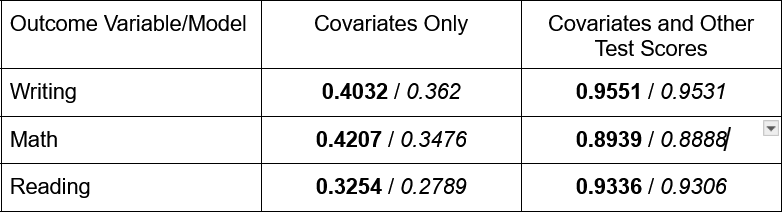
\includegraphics{Rsquared_tables.png}

Multiple \(R^2\) is bold, adjusted \(R^2\) is italicized.

\subsection{Table 3: Type B Model
Coefficients}\label{table-3-type-b-model-coefficients}

\subsubsection{Writing Score with Other Scores as
Predictors}\label{writing-score-with-other-scores-as-predictors}

\begin{longtable}[]{@{}lr@{}}
\toprule\noalign{}
Covariate & Coefficient \\
\midrule\noalign{}
\endhead
\bottomrule\noalign{}
\endlastfoot
(Intercept) & 1.8887616 \\
gendermale & -6.0578706 \\
ethnic\_groupgroup B & -0.4101061 \\
ethnic\_groupgroup C & 0.5802956 \\
ethnic\_groupgroup D & 2.1894542 \\
ethnic\_groupgroup E & -1.0099243 \\
parent\_educbachelor's degree & 0.9536092 \\
parent\_educhigh school & -1.4646427 \\
parent\_educmaster's degree & 2.4499005 \\
parent\_educsome college & 0.1507372 \\
parent\_educsome high school & -1.6961199 \\
lunch\_typestandard & 0.2287684 \\
test\_prepnone & -3.3650862 \\
parent\_marital\_statusmarried & 0.0939641 \\
parent\_marital\_statussingle & 0.2058865 \\
parent\_marital\_statuswidowed & 0.9320512 \\
practice\_sportregularly & 1.5653436 \\
practice\_sportsometimes & 0.8226377 \\
is\_first\_childyes & -0.2082400 \\
transport\_meansschool\_bus & -1.4653048 \\
wkly\_study\_hours\textgreater{} 10 & -0.3405180 \\
wkly\_study\_hours10-May & 0.0123796 \\
reading\_score & 0.7290976 \\
math\_score & 0.4190312 \\
transport\_meansschool\_bus:reading\_score & 0.0230636 \\
reading\_score:math\_score & -0.0016988 \\
\end{longtable}

The proper interpretation of these coefficients is as follows: Holding
all other variables constant, one unit increase in {[}covariate{]} leads
to {[}coefficient{]} units increase in the outcome of interest.

\subsection{Math Score with Other Scores as
Predictors}\label{math-score-with-other-scores-as-predictors}

\begin{longtable}[]{@{}lr@{}}
\toprule\noalign{}
Covariate & Coefficient \\
\midrule\noalign{}
\endhead
\bottomrule\noalign{}
\endlastfoot
(Intercept) & -9.4478352 \\
gendermale & 13.9310258 \\
ethnic\_groupgroup B & 0.9575902 \\
ethnic\_groupgroup C & -0.1500629 \\
ethnic\_groupgroup D & -0.8904819 \\
ethnic\_groupgroup E & 5.2158484 \\
parent\_educbachelor's degree & -1.3248714 \\
parent\_educhigh school & 0.6757209 \\
parent\_educmaster's degree & -3.2424452 \\
parent\_educsome college & 0.1386980 \\
parent\_educsome high school & 0.7638305 \\
lunch\_typestandard & 1.5110651 \\
test\_prepnone & 4.1051371 \\
parent\_marital\_statusmarried & 0.2781327 \\
parent\_marital\_statussingle & -0.1017812 \\
parent\_marital\_statuswidowed & 1.1956141 \\
practice\_sportregularly & 0.4596391 \\
practice\_sportsometimes & 0.0950948 \\
is\_first\_childyes & -1.5827564 \\
transport\_meansschool\_bus & 0.0626096 \\
wkly\_study\_hours\textgreater{} 10 & -4.9391993 \\
wkly\_study\_hours10-May & -2.9390114 \\
reading\_score & 0.1675506 \\
writing\_score & 0.7674974 \\
lunch\_typestandard:is\_first\_childyes & 2.5464054 \\
test\_prepnone:transport\_meansschool\_bus & -1.3404825 \\
wkly\_study\_hours\textgreater{} 10:reading\_score & 0.1000068 \\
wkly\_study\_hours10-May:reading\_score & 0.0554654 \\
\end{longtable}

The proper interpretation of these coefficients is as follows: Holding
all other variables constant, one unit increase in {[}covariate{]} leads
to {[}coefficient{]} units increase in the outcome of interest.

\subsection{Reading Score with Other Scores as
Predictors}\label{reading-score-with-other-scores-as-predictors}

\begin{longtable}[]{@{}lr@{}}
\toprule\noalign{}
Covariate & Coefficient \\
\midrule\noalign{}
\endhead
\bottomrule\noalign{}
\endlastfoot
(Intercept) & 2.2512938 \\
gendermale & -0.1377977 \\
ethnic\_groupgroup B & -0.1399523 \\
ethnic\_groupgroup C & -0.8456703 \\
ethnic\_groupgroup D & -2.1742851 \\
ethnic\_groupgroup E & -0.8495220 \\
parent\_educbachelor's degree & -0.3194345 \\
parent\_educhigh school & 0.9325487 \\
parent\_educmaster's degree & -0.9991043 \\
parent\_educsome college & -0.5342048 \\
parent\_educsome high school & 1.3485517 \\
lunch\_typestandard & -1.2290996 \\
test\_prepnone & 1.9926513 \\
parent\_marital\_statusmarried & 0.0740501 \\
parent\_marital\_statussingle & -0.1264861 \\
parent\_marital\_statuswidowed & -1.4360788 \\
practice\_sportregularly & -2.0714620 \\
practice\_sportsometimes & -0.7828685 \\
is\_first\_childyes & -0.6219640 \\
transport\_meansschool\_bus & 1.1396578 \\
wkly\_study\_hours\textgreater{} 10 & -0.3184942 \\
wkly\_study\_hours10-May & -0.1845646 \\
writing\_score & 0.8931576 \\
math\_score & 0.1209110 \\
is\_first\_childyes:transport\_meansschool\_bus & 1.5524335 \\
transport\_meansschool\_bus:writing\_score & -0.0297898 \\
\end{longtable}

The proper interpretation of these coefficients is as follows: Holding
all other variables constant, one unit increase in {[}covariate{]} leads
to {[}coefficient{]} units increase in the outcome of interest.

\subsection{Explore Diagnostics for These
Models}\label{explore-diagnostics-for-these-models}

\subsubsection{Figure 1: Diagnostic plots for the Writing Type A
Model}\label{figure-1-diagnostic-plots-for-the-writing-type-a-model}

\includegraphics[width=0.9\linewidth]{Mari_Work_files/figure-latex/unnamed-chunk-26-1}

\subsubsection{Figure 2: Diagnostic plots for the Math Type A
Model}\label{figure-2-diagnostic-plots-for-the-math-type-a-model}

\includegraphics[width=0.9\linewidth]{Mari_Work_files/figure-latex/unnamed-chunk-27-1}

\subsubsection{Figure 3: Diagnostic plots for the Reading Type A
Model}\label{figure-3-diagnostic-plots-for-the-reading-type-a-model}

\includegraphics[width=0.9\linewidth]{Mari_Work_files/figure-latex/unnamed-chunk-28-1}

\subsubsection{Figure 4: Diagnostic plots for the Writing Type B
Model}\label{figure-4-diagnostic-plots-for-the-writing-type-b-model}

\includegraphics[width=0.9\linewidth]{Mari_Work_files/figure-latex/unnamed-chunk-29-1}

\subsubsection{Figure 5: Diagnostic plots for the Math Type B
Model}\label{figure-5-diagnostic-plots-for-the-math-type-b-model}

\includegraphics[width=0.9\linewidth]{Mari_Work_files/figure-latex/unnamed-chunk-30-1}

\subsubsection{Figure 6: Diagnostic plots for the Reading Type B
Model}\label{figure-6-diagnostic-plots-for-the-reading-type-b-model}

\includegraphics[width=0.9\linewidth]{Mari_Work_files/figure-latex/unnamed-chunk-31-1}

\end{document}
